\documentclass{IEEEtran}
\usepackage[spanish]{babel} % Definir el idioma del documento
\usepackage[letterpaper,top = 2cm, bottom = 2cm, left = 2cm, right = 2cm, marginparwidth = 1.75cm]{geometry} % Especificar los márgenes según la norma
\usepackage{pdfpages} % Añadir PDFs y que te cuente las páginas para el documento
\usepackage{subfiles} % Tener subdocumentos (hay más opciones)
\usepackage{tableof} % Se utiliza para los indices de los subdocumentos
\usepackage{float} % Para usar lo de 'H'
\usepackage{fancyhdr}
\usepackage{comment}
\usepackage{biblatex} % Paquete para manejar citas y bibliografía
\usepackage{amsmath}
\addbibresource{bibliografia.bib} % Cargar el archivo .bib

\def\TituloProyecto{Puente de Cody Docks}
\def\Autor{Mercedes Román Ruiz}
\def\Asignatura{Ampliación de Mecánica}
\def\Curso{2024 - 25}
\def\Fecha{Mayo 2024}

\begin{document}
\sloppy 
\setlength{\parindent}{30pt}
\setlength{\parskip}{6pt}
\renewcommand\thesection{\arabic{section}}
\renewcommand{\baselinestretch}{1.5}

\begin{titlepage}
    \centering
    
\includegraphics[width=0.5\linewidth]{Imagenes/Logo UPM.png} \par
    \vspace{1cm}
    {\bfseries\LARGE Escuela Técnica Superior de Ingenieros Industriales \par}
    \vspace{0.5cm}
    {\scshape\Large Máster en Ingeniería Industrial \par}
    \vspace{3 cm}
    {\Huge \textbf{\TituloProyecto} \par}
    \vfill
    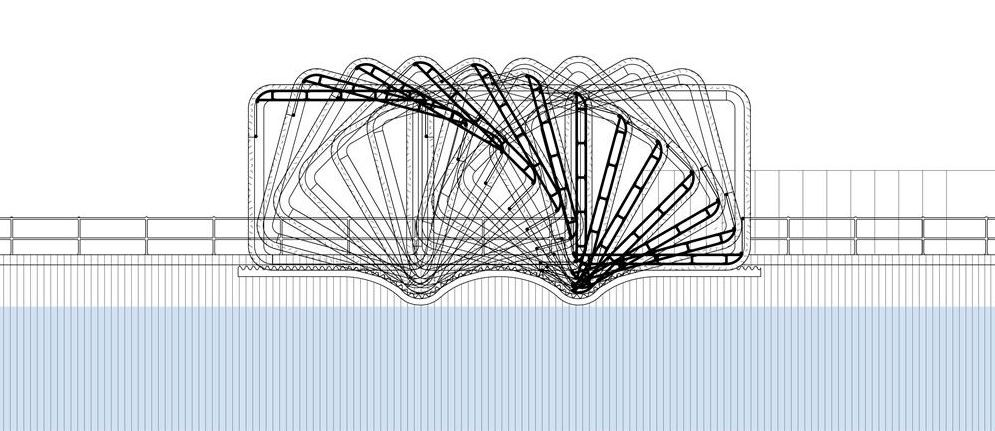
\includegraphics[width=0.5\linewidth]{Imagenes/Puente de Cody Docks.jpg} \par
    \vfill
    {\Large Autora: Mercedes Román Ruiz \par}
    {\Large \Asignatura \  \Curso \par}
    {\Large \Fecha \par}
\end{titlepage}

\tableofcontents

\section{Introducción}

El Puente Rodante de Cody Dock, diseñado por Thomas Randall-Page, constituye un avance significativo en la ingeniería de puentes móviles, destacando por su innovador sistema de rodadura completa. Concebido como una solución ingeniosa para las limitaciones espaciales y presupuestarias propias del entorno urbano de Londres, este puente logra rotar sobre sí mismo para permitir el paso de embarcaciones, prescindiendo de la necesidad de motores eléctricos o sistemas hidráulicos. Esta característica lo distingue de los diseños convencionales y subraya su eficiencia en contextos urbanos densos.

La singularidad del diseño del Puente de Cody Dock radica en su fundamentación en principios matemáticos establecidos. En 1849, James Clerk Maxwell descubrió que una línea recta rueda suavemente sobre una catenaria invertida. Posteriormente, en 1960, G. Robison extendió esta idea al demostrar que un cuadrado puede rodar suavemente sobre una secuencia de catenarias truncadas y unidas. Para visualizar y demostrar este concepto, Stan Wagon construyó un triciclo de tamaño completo en 1997, alcanzando una gran repercusión mediática (Fig. \ref{fig: Ripley's Belive It or Not}). Estos descubrimientos teóricos proporcionaron la base para que Randall-Page concibiera el Puente de Cody Dock como una plataforma unida a dos grandes cuadrados, permitiendo que la estructura complete una rotación suave hasta una posición invertida. 

Los puentes móviles tradicionales, tales como los levadizos o basculantes, frecuentemente imponen exigencias significativas en términos de espacio, tanto vertical como horizontal, para su operación. Además, estos diseños suelen requerir la implementación de sistemas mecánicos complejos, lo que se traduce en costes elevados tanto en la fase de construcción como en el mantenimiento a largo plazo. En entornos urbanos consolidados, donde el espacio es un recurso escaso y valioso, estas soluciones pueden resultar poco prácticas. El Puente Rodante de Cody Dock emerge como una alternativa eficaz y eficiente, ofreciendo una solución que minimiza la ocupación de espacio y que, gracias a su diseño innovador, facilita la apertura del paso fluvial mediante una rotación manual controlada del cuerpo del puente.

\begin{figure}[h]
    \centering
    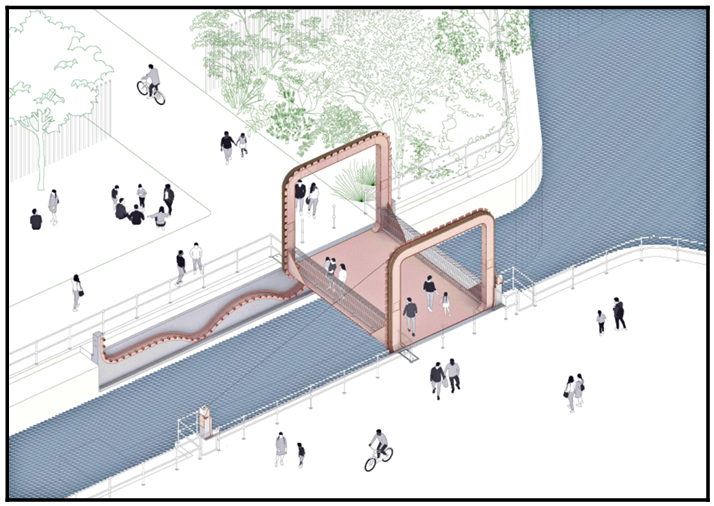
\includegraphics[width = 0.5 \textwidth]{Imagenes/Cody Dock Sketch.png}
    \caption{Boceto del Puente - Thomas Randall-Page \cite{randallpage2021}.}
    \label{fig: Dibujo de Cody Dock}
\end{figure}

\begin{figure}[h]
    \centering
    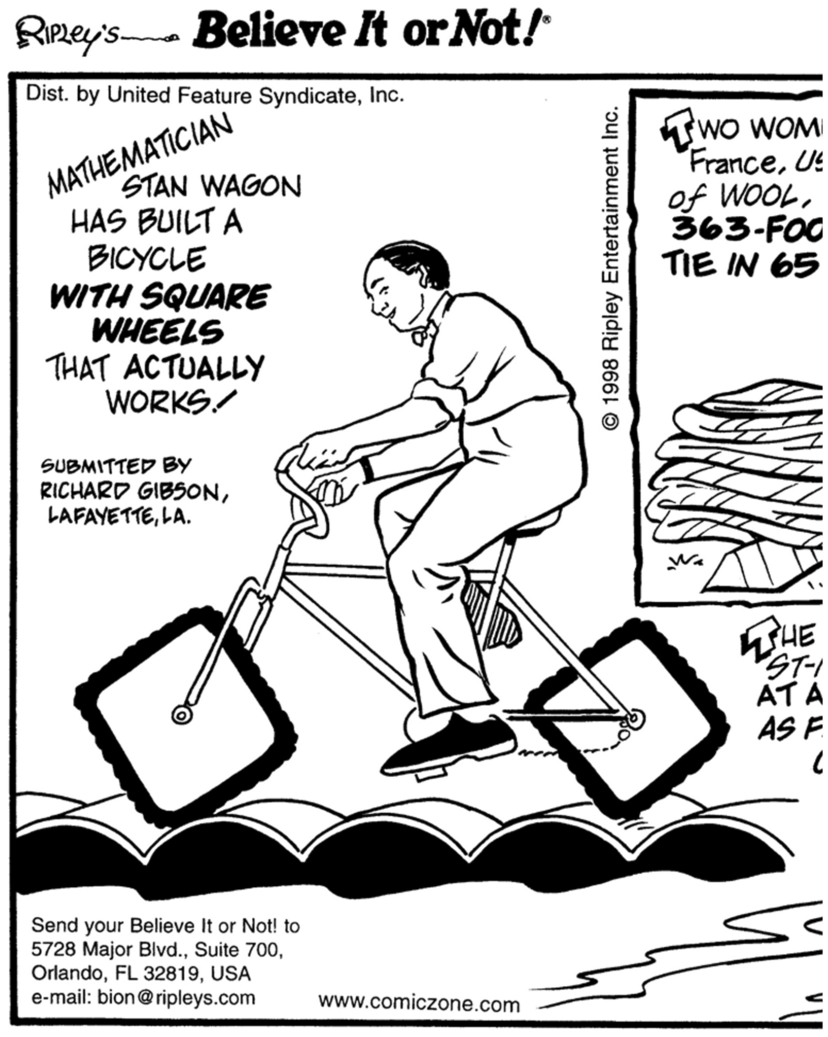
\includegraphics[width = 0.5 \textwidth]{Imagenes/Square Wheel Tricycle.png}
    \caption{Publicación sobre la bicicleta de rueda cuadrada en Ripley's Belive It or Not.}
    \label{fig: Ripley's Belive It or Not}
\end{figure}

\section{Teoría del Rodamiento de Curvas}

En su artículo \textit{``On the Theory of Rolling Curves''}, presentado a la Royal Society of Edinburgh en 1849, James Clerk Maxwell exploró las propiedades geométricas de las curvas generadas por el rodamiento de una curva sobre otra, sentando las bases para aplicaciones posteriores como el puente de Cody Dock. 

Cuando la rueda es un círculo perfecto ($r(\theta) = 1$), su movimiento describe una relación simple: la posición horizontal sigue $x(\theta) = \theta + \frac{\pi}{2}$ mientras rueda sobre una carretera plana ($y = -1$). Sin embargo, Maxwell analizó un caso más intrigante: una rueda constituida por una línea recta infinita ($x = -1$) con centro de masa en el origen $(0,0)$. En sus propias palabras: 

\begin{quote}
``La línea recta cuya ecuación es $r = a \sec \theta$, rodando sobre una catenaria cuyo parámetro es $a$, traza una línea cuya distancia desde el vértice es $a$''.
\end{quote}

El término \textit{``traza''} aquí se refiere al lugar geométrico del origen (centro de masa) a medida que la línea rueda. Para una línea horizontal expresada en coordenadas polares como $r = -\csc \theta$ (con $-\pi < \theta < 0$), la forma de la carretera se obtiene integrando:

\[
x(\theta) = \int_{-\pi/2}^{\theta} -\csc t \, dt = \ln\left(-\cot\left(\frac{\theta}{2}\right)\right).
\]

Esta expresión paramétrica puede transformarse a la forma explícita $y = f(x)$. Primero, al invertir la relación se obtiene $\theta = -2 \tan^{-1}(e^{-x})$. Sustituyendo en la ecuación de la carretera, $y = -\csc \theta$, se revela la identidad fundamental:

\[
y = -\cosh x,
\]

que corresponde exactamente a una catenaria invertida. La figura \ref{fig: A line rolling along a catenary} muestra la línea rodando. Este resultado, aunque elegante, no incluyó en su momento la posibilidad de truncar la línea recta para crear ruedas poligonales, una idea que surgiría un siglo después con los trabajos de Robison y su aplicación en el puente de Cody Dock.

\begin{figure}[h]
    \centering
    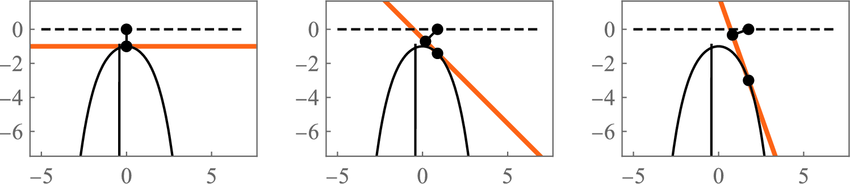
\includegraphics[width = 0.5 \textwidth]{Imagenes/A line rolling along a catenary.png}
    \caption{Línea que rueda a lo largo de una catenaria.}
    \label{fig: A line rolling along a catenary}
\end{figure}

\section{Una rueda cuadrada}

En 1960, Robinson redescubrió el resultado de Maxwell y lo extendió para diseñar una rueda de forma cuadrada. Su idea innovadora consistió en truncar la catenaria en los puntos donde su pendiente es $\pm 1$. En dichos puntos, la catenaria forma un ángulo de $45^\circ$ con la vertical, lo que permite que, al colocar una copia truncada de la catenaria junto a otra, se genere una cúspide de $90^\circ$ que encaja perfectamente con la esquina de un cuadrado (Figura \ref{fig: A square rolls smoothly along linked catenaries}).

Como la derivada de $\cosh x$ es $\sinh x$, las cúspides ocurren cuando $x = \pm \sinh^{-1}(1)$, es decir, aproximadamente en $\pm 0.88$. De este modo, el cuadrado puede rodar sobre esta carretera manteniendo su centro de masa a una altura constante. Esto implica que el movimiento no realiza trabajo contra la gravedad y, en esencia, es dinámicamente equivalente al de un círculo rodando sobre una superficie plana.

Este modelo permite construir tanto la carretera como una rueda cuadrada que se desplace de manera sorprendentemente suave. Un aspecto técnico relevante es que la relación entre $x$ (posición horizontal) y $\theta$ (parámetro angular) no es lineal. En consecuencia, si se aplica una velocidad angular constante al cuadrado, el avance horizontal no será uniforme. Sin embargo, dicha relación es lo suficientemente cercana a la linealidad como para que esta variación no resulte perceptible en la práctica.

\begin{figure}[h]
    \centering
    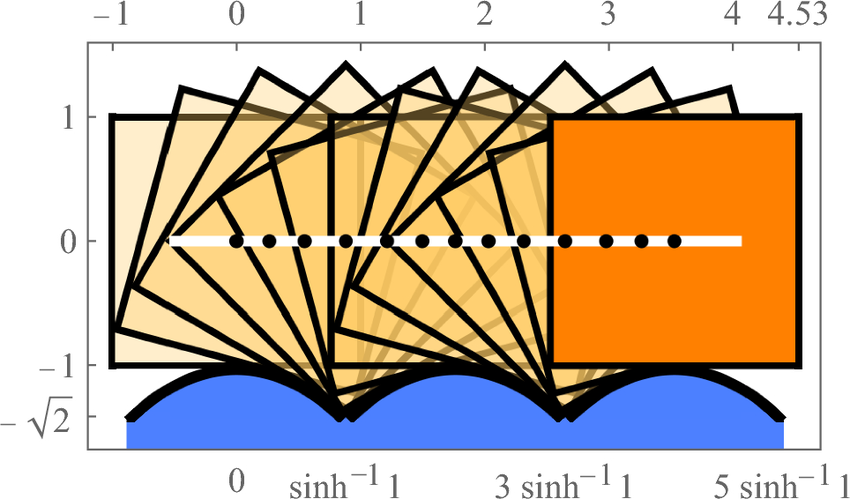
\includegraphics[width = 0.5 \textwidth]{Imagenes/A square rolls smoothly along linked catenaries.png}
    \caption{Cuadrado rodando suavemente a lo largo de catenarias conectadas.}
    \label{fig: A square rolls smoothly along linked catenaries}
\end{figure}

\section{Las Matemáticas del Puente de Cody Dock}

El puente de Cody Dock utiliiza dientes y pasadores para guiar la estructura rodante de acero, y para que estos encajen, los ángulos rectos deben ser eliminados. Esto se logra redondeando las esquinas de la manera más natural: usando cuartos de círculo.

Consideremos una rueda de radio $1$, con centro de masa en el origen $(0, 0)$ y centro geométrico en $(0, y_0)$, donde $y_0 \leq -1$. Dado que el origen está fuera del círculo, no es posible describir toda la rueda en forma polar. En su lugar, se representa paramétricamente como $g(t) = (g_1(t), g_2(t))$. Por tanto, la parametrización de la carretera sobre la que rodará es:

\[ x(t) = \int_{0}^{t}{\frac{g_1(s) g_2'(s) - g_1'(s) g_2(s)}{\sqrt{g_1(s)^2 + g_2(s)^2}}} \]
\[ y(t) = - \sqrt{g_1(t)^2 + g_2(t)^2} \]

Para nuestra rueda circular, $g(t) = (sin t, y_0 - \cos t)$, lo que lleva a:

\[ x(t) = \int_{0}^{t}\frac{1 - y_0 \cos s}{\sqrt{1 + y_0^2 - 2 y_0 \cos s}} \]
\[ y(t) = - \sqrt{1 + y_0^2 - 2 y_0 \cos t} \]

Para evaluar esta integral, se realiza un cambio de variable $s = \frac{\pi}{2} - u$, convirtiendo cosenos en senos. Tras una seria de manipulaciones algebraicas y el uso de integrales elípticas $E$ y $F$, se obtiene la solución:

\[ x(t) = (1 - y_0) E \left( \frac{t}{2} | - \frac{4y_0}{(1 - y_0)^2} \right) + (1 + y_0) F \left( \frac{t}{2} | - \frac{4 y_0}{(1 - y_0)^2} \right) \]

\[ y(t) = - \sqrt{1 + y_0^2 - 2 y_0 \cos t} \]

La carretera resultante es una secuencia de bucles. Aunque esto imposibilita construir un modelo físico completo, el puente solo requiere una pequeña porción de esta estructura para las esquinas redondeadas.

Para el puente, la carretera es una curva compuesta que combina segmenteos de catenarias ($y = - \cosh x)$ para las rectas y segmentos de los bucles para las esquinas redondeadas. Un enfoque simplificado permite calcular esta curva usando solo la integral elíptica $E$, lo que fue crucial para el diseño final.

\section{Contexto Urbano e Histórico}
Cody Dock se ubica en el East London, a lo largo del río Lea, una zona industrial en transformación hacia un espacio comunitario y ecológico. El área requería una conexión peatonal permanente y, al mismo tiempo, permitir el paso ocasional de embarcaciones por el canal. La intervención se enmarca en un proceso de regeneración urbana, con fuerte participación ciudadana y financiación colectiva. El diseño debía cumplir con criterios de bajo impacto, mantenimiento mínimo y alta fiabilidad.

\section{Principios de Funcionamiento y Diseño}
\subsection{Geometría estructural}
La estructura está formada por una sección tubular circular de acero, construida mediante perfiles huecos soldados. El radio de curvatura del puente coincide con el de los rieles de soporte, generando una rotación suave sobre un eje horizontal. La geometría fue cuidadosamente optimizada para mantener el centro de masas dentro del radio de rodadura, facilitando la operación manual.

\subsection{Mecanismo de rodadura}
El puente gira sobre dos rieles semicirculares mediante un sistema de engranajes y manivelas, sin necesidad de sistemas electrónicos ni motores. El momento necesario para la rotación se reduce mediante contrapesos y equilibrado estructural.

\section{Análisis Mecánico y Estructural}
\subsection{Modelo simplificado}
La estructra puede analizarse como un cilindro hueco sometido a cargas distribuidas por peso propio y carga peatonal. Usando modelos de elementos finitos se verificó que la estructura resiste adecuadamente las fases de carga máxima en posición horizontal y durante la rotación.

\subsection{Momentos y esfuerzos}
Se identificaron puntos críticos de concentración de tensiones en las zonas de apoyo sobre los rieles y en las uniones de los eleemntos estructurales. Se utilizaron conectores soldados con refuerzos triangulares para distribuir las cargas.

\section{Materiales y Construcción}
\subsection{Material principal}
El puente está fabricado principalmente en acero estructural S275, que presenta buena resistencia mecánica, soldabilidad y comportamiento a fatiga. El tablero es de madera reciclada, tratada con compuestos impermeabilizantes.

\subsection{Proceso de montaje}
Los componentes estructurales fueron prefabricados en taller y transportados al sitio para su ensamblaje. El sistema modular permitió una construcción rápida con mínima maquinaria pesada. La cimentación se realizó con bloques de hormigón armado, donde se fijaron los rieeles de rodadura.

\section{Análisis de Sostenibilidad}
La solución propuesta destaca por su bajo consumo energético durante la operación, ya que es completamente manual. Además se emplearon materiales reciclados y se redujo el impacto ambiental durante la construccuón. El mantenimiento es mínimo y puede ser realizado por personal no especializado.

\section{Participación Comunitaria}
Uno de los aspectos más destacados del proyecto fue la inclusión de la comunidad local tanto en la fase de diseño como en la construcción. Voluntarios colaboraron en el montaje del puente, y actualmente participan en su operación diaria. Esto fortalece el sentido de pertenencia y el cuidado de equipamiento urbano.

\section{Limitaciones y Consideraciones Técnias}
Entre las limitaciones del sistema destacan:
\begin{itemize}
    \item No es apto para tráfico rodado pesado.
    \item Requiere inspecciones periódicas para prevenir la corrosión del acero.
    \item La operación manual puede no ser viable en caso de discapacidad o climas extremos.
\end{itemize}

Se recomienda su uso principalmente para zonas peatonales, vías verdes y entornos urbanos con bajo tráfico.

\section{Potencial de Replicabilidad}
El diseño puede adaptarse a otras localizaciones modificando su escala, materiales o modo de operación. Su bajo coste y simplicidad constructiva lo convierten en una opción viable para proyectos de regeneración urbana o de movilidad sostenible.

\section{Conclusión}
El Puente Rodante de Cody Dock ejemplifica una aproximación innovadora al diseño de infraestructuras urbanas móviles. Combinando principios básicos de la mecánica clásica con objetivos sociales y medioambientales, constituye una referencia para futuras intervenciones de ingeniería con enfoque comunitario y sostenible.

\nocite{*}
\printbibliography

\end{document}